\section{Prospective workflow pilot}
\label{app:pilot}
The pilot used the pinned $\tau^2$-bench source revision
\texttt{b7ea9074c1cb} (full hash in the protocol) and its base telecom
tasks. From tasks with deterministic action/environment criteria and no
natural-language grading assertion, we selected the twelve lowest hashes
of the master seed 20260918 and task identifier. The complete tasks,
selection, randomized within-task workflow order, independent arm seeds,
model identifiers and exact verification prompt were frozen in a dated
local protocol before model outputs were collected. This is a laboratory
workflow experiment with simulated users, not production-user A/B testing.

An initial protocol compared GPT-5.6-Luna and Claude Haiku 4.5, with a
common Luna user simulator. Its first request failed for exhausted
OpenAI quota, yielding no completed trajectory. The original protocol,
zero-completion records and \$0.0078588 retained reservation remain
immutable. Before collecting any completed output, we recorded an
infrastructure-motivated amendment: standard versus verification-prompt
workflows, both using \texttt{claude-haiku-4-5-20251001}, with the same
Haiku user simulator in both arms. The twelve tasks and mapped randomized
order were retained. No task, prompt, step or monetary limit was changed
after observing the amended pilot's outcomes.

The standard agent uses the upstream default system prompt and telecom
policy. The additional verification instruction asks the agent to check
the applicable policy and observed state before a state-changing tool
call, verify corrective actions with available diagnostics or specific
user confirmation, and avoid declaring resolution without an observable
check. It explicitly does not override domain policy. Both workflows use
temperature zero, at most 40 steps, four errors, output limits of 384
agent tokens and 192 user-simulator tokens, and one trial per task and
workflow. Provider randomness is not guaranteed reproducible by the
simulator seeds. API calls use direct transport with zero retries and no
model fallback. A conservative reservation precedes each request; actual
reported usage is then priced at the frozen list rates. Uncertain failed
requests retain their reservation, and an unaffordable next request stops
the experiment. These constraints are part of the evaluated workflow.

There were 484 completed amended-pilot requests. Eighteen trajectories
completed on nine task pairs; the next trajectory stopped before a request
could fit the remaining reservation budget, and the remaining planned
records were retained as unobserved. Standard and verification each had
two successes, seven completed failures, six step-cap terminations and
three unobserved planned runs. Among the nine complete pairs, verification
had zero wins, two losses and seven ties. Complete-case net preference
$-2/9$ is descriptive only: stopping on cumulative cost can select which
tasks are completed. The full planned cohort therefore remains explicit.

If the known score sum over $m$ of $N=12$ pairs is $s$, each unknown
pair lies in $[-1,1]$, giving deterministic support bounds
$[(s-(N-m))/N,(s+(N-m))/N]$. With $s=-2,m=9$ these are
$[-5/12,1/12]$ for the planned-cohort net preference. The observed success
difference sum is zero, yielding $[-3/12,3/12]$. These conservative bounds
ignore partial one-arm information. They express missing finite-cohort
outcomes, not population sampling uncertainty or a confidence sequence.

The amended pilot's usage-priced list cost was \$3.937767. Including the
retained initial reservation gives \$3.9456258 under the combined \$4 cap.
Two separate provider diagnostics account for \$0.002035, so the total
project ledger is \$3.9476608 under its initial \$5 allocation. These are
conservative usage/reservation accounts, not reconciled provider invoices.
Credentials and private raw text are excluded from release. Sanitized
trace metadata, tool names, text hashes, token use, task checks, complete
planned-run records, frozen source hashes, and the cost ledger permit
inspection of the reported summaries.

\begin{figure}[h]
\centering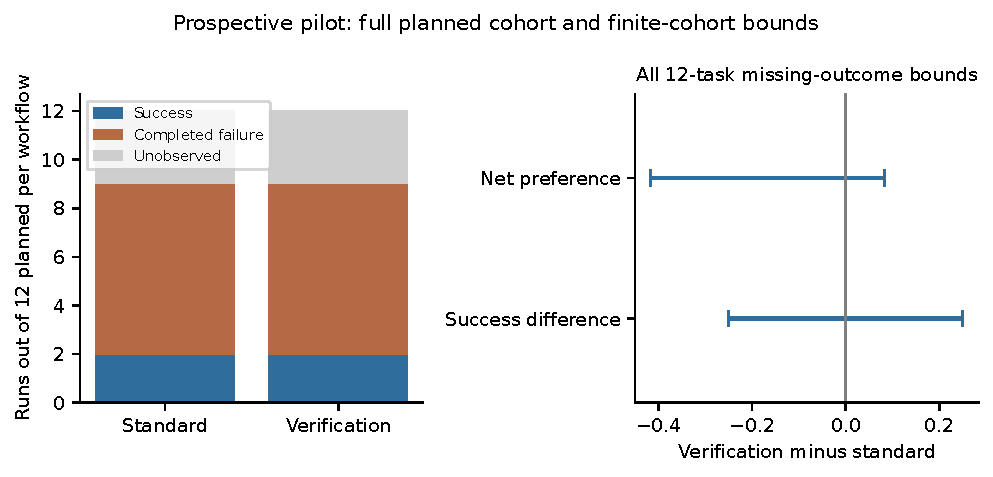
\includegraphics[width=\linewidth]{../plots/prospective_v2_cohort.pdf}
\caption{Prospective laboratory feasibility pilot. All planned tasks,
including unobserved runs, remain in the cohort. Horizontal intervals
are deterministic missing-outcome bounds, not sampling confidence intervals.}
\end{figure}
